\begin{figure}[H]
    \center
    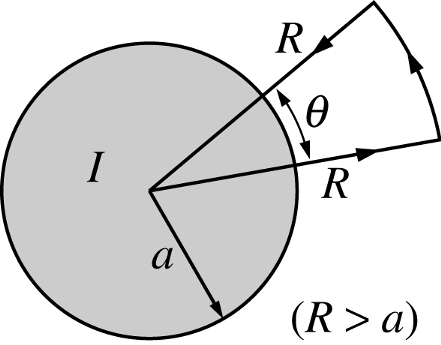
\includegraphics[scale=0.25]{images/img-013-025.png}
\end{figure}

% Multiple Choice Question 35
\begin{questions}\setcounter{question}{34}\question
A long, straight wire of radius $a$ carries a current $I$ out of the page, which is uniformly distributed over the cross section of the wire. The value of $\oint \mathbf{B} \cdot \diff \boldsymbol{\ell}$, the line integral of the magnetic field
$\mathbf{B}$ around the wedge-shaped path, equals which of the following?

\begin{oneparchoices}
\choice $\dfrac{\mu_{0} \theta I}{2 \pi}$
\choice $\dfrac{\mu_{0} \theta I}{2 \pi^{2} a^{2}}$
\choice $\dfrac{\mu_{0} \theta I}{2 \pi^{2} R^{2}}$
\choice $\dfrac{\mu_{0} I}{\pi a^{2}}$
\choice $\dfrac{\mu_{0} I}{\pi R^{2}}$
\end{oneparchoices}\end{questions}

